\documentclass[]{ceurart}

\sloppy
\usepackage{listings}
\lstset{breaklines=true}
\usepackage{longtable}
\usepackage{float}
\usepackage{etoolbox}
\providecommand{\tightlist}{\setlength{\itemsep}{0pt}\setlength{\parskip}{0pt}}
\providecommand{\pandocbounded}[1]{#1}
\usepackage{graphicx}
\usepackage{booktabs}
\usepackage{caption}
\usepackage{longtable}
\usepackage{colortbl}
\usepackage{array}
\usepackage{anyfontsize}
\usepackage{multirow}
\makeatletter
\@ifpackageloaded{caption}{}{\usepackage{caption}}
\AtBeginDocument{%
\ifdefined\contentsname
  \renewcommand*\contentsname{Table of contents}
\else
  \newcommand\contentsname{Table of contents}
\fi
\ifdefined\listfigurename
  \renewcommand*\listfigurename{List of Figures}
\else
  \newcommand\listfigurename{List of Figures}
\fi
\ifdefined\listtablename
  \renewcommand*\listtablename{List of Tables}
\else
  \newcommand\listtablename{List of Tables}
\fi
\ifdefined\figurename
  \renewcommand*\figurename{Figure}
\else
  \newcommand\figurename{Figure}
\fi
\ifdefined\tablename
  \renewcommand*\tablename{Table}
\else
  \newcommand\tablename{Table}
\fi
}
\@ifpackageloaded{float}{}{\usepackage{float}}
\floatstyle{ruled}
\@ifundefined{c@chapter}{\newfloat{codelisting}{h}{lop}}{\newfloat{codelisting}{h}{lop}[chapter]}
\floatname{codelisting}{Listing}
\newcommand*\listoflistings{\listof{codelisting}{List of Listings}}
\makeatother
\makeatletter
\makeatother
\makeatletter
\@ifpackageloaded{caption}{}{\usepackage{caption}}
\@ifpackageloaded{subcaption}{}{\usepackage{subcaption}}
\makeatother

\begin{document}

\copyrightyear{2026}
\copyrightclause{Copyright for this paper by its authors.
  Use permitted under Creative Commons License Attribution 4.0
  International (CC BY 4.0).}

\conference{Proceedings of the Workshop on Augmented Democracies (AuDe),
co-located with IJCAI-ECAI 2026}

\title{When LLMs agents Deliberate}
\tnotemark[1]
\tnotetext[1]{The work benefited from funding in the Horizon Europe
project ``European City Squared'' (Grant agreement ID:
\href{https://doi.org/10.3030/101178170}{101178170}).}

\author[1]{Jan Lorenz}[%
orcid=0000-0002-5547-7848,%
email=jlorenz@constructor.university,%
]

\author[1]{Erkan Gunes}[%
orcid=0009-0005-8106-3314,%
email=eguenes@constructor.university,%
]


\address[1]{Constructor University, Bremen, Germany}

\begin{abstract}
Deliberation is a democratic process helping to translate citizen
preferences to policy not by aggregating preferences but through
preference changes ideally towards a consensus. Nowadays, AI-augmented
human deliberators can be assisted by Large-Language Models (LLMs).
However, deliberation can also contribute to separating deliberators
into groups with opposing worldviews even more than before deliberation.
We study such deliberation processes using an agent-based model where
core decisions about changes in worldview are made by LLMs. In the
model, agents continually encounter new worldview statements through a
joint news channel or their social networks. They decide what to accept,
remember, reject, or share. Over time, these choices reshape individual
worldviews and generate collective patterns such as consensus,
polarization, or filter bubbles. Unlike persona-based simulations,
agents are not assigned demographic profiles or ideological labels, but
their worldviews develop through repeated exposure, integration,
replacement of worldview statements. In this first version of the model
we work with a limited set of hundred statements which are all derived
from the World Values Survey 2018 questionnaire. Preliminary results
produce collective patterns, including convergence around common
statements, concentration of attention on a narrow subset of the
statement pool, and separation into rival worldview clusters. Early
comparisons suggest that information sharing modes and memory capacity
may shape whether collective attention narrows around a few statements
or preserves diversity for competing clusters. These findings connect
individual information choices to emergent population level worldviews.
\end{abstract}

\begin{keywords}
agent-based models \sep large-language models \sep filter
bubbles \sep opinion dynamics
\end{keywords}

\maketitle

\section{Introduction}\label{introduction}

Deliberative processes are essential to ensuring the effective
translation of citizen preferences to policy. Studying the dynamics of
opinion change and stability at micro and macro scales can help
identifying the conditions under which deliberation produces informed
and coherent collective outcomes. This project focuses on how
individuals' views may change, stabilize, or become more isolated as
they encounter opinionated statements through different information
channels. We are particularly interested in the emergence of filter
bubbles and polarization as a result of repeated exposure to statements
flowing into an agent's feed from news media and social networks. We use
LLMs to mimic human behavior in a simplified way. In an AI-augmented
democracy, human deliberators may be assisted by LLMs, or deliberation
may be fully outsourced to LLMs representatives. Therefore, it is also
of interest to understand the dynamics of deliberating LLMs.

Agent-based models (ABM) are useful tools for studying opinion dynamics
and implications for deliberative processes, especially for explaining
the emergence of macro level phenomena such as filter bubbles.
Conventional opinion dynamics ABMs often represent opinions as points in
a low-dimensional numerical space where distance between two points
measures the difference of opinion
\citet{GeschkeEtAl2019TriplefilterBubbleUsing}. Our approach in this
project instead uses natural language opinion statements, and agents
that can understand and act on natural language statements. Statements
transform from points in two-dimensional numerical space to textual
statements. Instead of linking to numerical positions, agents maintain a
list of statements as their worldview. The behavioral mechanisms of
integrating and dropping statements are prompted to an LLM. The LLM
responds with a structured output and the agent's integration and
dropping decisions can be executed in the simulation timeline.

Technically, the model consists of agents embedded in a social network
where all agents are initialized with a fixed number of opinion
statements. Each agent has a bounded memory containing a limited number
of opinion statements, which together represent that agent's worldview.
Statements originate from a statement pool, which is built using the
World Values Survey questionnaire as the basis. At each time step,
agents are exposed to statements from a shared feed and/or to statements
circulated by their network neighbors. In both cases they then decide
whether to integrate one of these statements into memory or reject all
candidate statements. If their memory is full, adopting a new statement
requires dropping an existing one. Agents can share statements from
their own memory with their neighbors.~

Our approach differs from persona-based LLM simulations, which has been
the preferred approach to simulating human behavior with LLMs
\citep{ArgyleEtAl2023OutOneMany, PromaEtAl2026CanLLMsEmulate}. Rather
than assigning agents fixed demographic profiles or ideological labels,
and instructing them to return responses to a set of behavioral
questions, we represent their worldview as an evolving memory of
statements and ask them to accept or reject new statements given their
worldview at the time of decision. Agents are not predefined as
liberals, conservatives, moderates, or members of specific social
groups. Their worldviews develop through repeated exposure, uptake,
replacement, and sharing. This matters for deliberation research because
deliberation is precisely a process through which preferences and
identities may change.

Opinion dynamics is an established and a prominent approach to
agent-based modeling of socio-political systems
\citep{FlacheEtAl2017ModelsSocialInfluence, LorenzEtAl2021IndividualAttitudeChange}.
Models of opinion dynamics have been used to understand the mechanisms
of societal radicalization and polarization, and the emergence of filter
bubbles in various ways
\citep{KeijzerMaes2022ComplexLinkFilter, KeijzerEtAl2026ComputationalSocialScience}.
A shortcoming of opinion dynamics models has always been that something
as complex as the opinion of a human being has to be boiled down to one
number or to a vector of few numbers in an abstract numerical opinion
space such as the left-right political continuum.

While numerical opinion spaces may seem disconnected with the reality of
how opinions exist in the real world, they are not arbitrary model
design choices. Researchers measure individuals' attitudes through
representative surveys, where individuals self-assess their attitudes on
numerical or categorical scales. In addition, actors in political
discourse in the real world use spatial metaphors such as a politician
moving to the right, left, or center. Accordingly, political science has
developed several methods for positioning political actors and texts in
low-dimensional numerical opinion spaces. These methods range from
expert assessments using theory-driven classification to data-driven
approaches measuring positions in latent dimensions of
higher-dimensional spaces using roll-call, co-voting data, survey data,
or texts using dimensionality reduction and natural language processing.
The well-known models of continuous opinion dynamics
\citep[see][]{Lorenz2025ExploringTheoryAgentbased} make use of such
abstract low-dimensional opinion spaces and define how individuals
change their opinion on that scale when confronted with the opinions of
others. However, in reality, an attitude change does not occur based on
the exchange of numerical numbers but through verbalization of arguments
\citep{BanischOlbrich2019OpinionPolarizationLearning}, persuasive
messages, and emotional emphasis, whether written or spoken language, or
other media such as images. While it is plausible that the attitudes of
individuals can be mapped reasonably well into a low-dimensional
numerical space for descriptive purposes, it is less realistic that
individual attitude change can be well operationalized solely based on
just the exchange of numbers.

Large Language Models (LLMs) provide a new opportunity to build a new
generation of opinion dynamics models. LLMs trained on large bodies of
text seem to have embedded the meaning of the antagonisms and
compatibilities of opinions as stated in written texts. In this paper,
we build such a model inspired by the filter bubble model of
\citet{GeschkeEtAl2019TriplefilterBubbleUsing}. The main entities in
their model are agents positioned in a two-dimensional numerical opinion
space, and opinionated statements represented by \emph{bits of
information} which are also points in the the same opinion space. Agents
are linked to a limited number of bits of information which together
represent their worldview. Their positions are defined by the
coordinates in the opinion space that correspond to the average position
of their worldview. Further on, agents maintain a social network of
bidirectional friendship links. Based on this setup, agents have a few
behavioral mechanisms implemented. When they are presented with a new
point in opinion space, either from a central media channel or their
friends, they decide whether to integrate it into their worldview or
not. If they integrate it they drop another bit of information. With a
change of bits of information they adjust their position in opinion
space to the new worldview average. They can share a bit of information
of their worldview along all their friendship links, mimicking its
posting on social media.

The macroscopic opinion landscape of agents and statements in the model
is thus a bipartite network of agents and statements, where agents are
linked to the bits of information of their worldview, and bits of
information are linked to the agents that have them in their worldview.
In such an opinion landscape, a \emph{bubble} is a set of agents whose
worldviews have a high overlap of statements while the overlap with all
other agents is low or non-existent.

The model shows emergent phenomena and how they depend on model
parameters. Firstly, when new bits of information comes in from a
central media source which every agent can see, the opinion landscape
develops a structure characterized by high and low density regions but
the network remains fully connected without strong bubbles. Secondly,
when agents are able to see statements shared by friends, the opinion
landscape develops a structure characterized by bubbles. Thirdly, how
many bubbles emerge depends to a large extent on a parameter called
latitude of acceptance which defines how far away a statement can be
from the average position of an agent's worldview to be integrated. When
this latitude is small, many small bubbles emerge. When it is large
enough, only one large bubble emerges.

We transform this model into a text-based setup without a numerical
opinion space. Statements transform from dots (information bits) in
two-dimensional numerical space to textual opinionated statements.
Instead of linking to numerical positions, agents maintain a list of
statements in their memory as their worldview. The behavioral mechanisms
of integrating and dropping statements are performed by LLM agents based
on instructions passed to them through their system prompt.

In this study, we use a limited set of 100 statements extracted from the
World Values Survey questionnaire. Each statement is directly related to
one survey item and to a certain response or response scale. This
approach facilitates the validation of emerging worldviews in LLM
simulations with real survey responses.

The phenomena we aim to study with this model are on different levels.
On macro level phenomena our main questions focus on whether the textual
representation of opinions and the use of LLMs for integration and
dropping decisions lead to a similar bubble formation phenomena as the
numerical model, whether the presence or absence of social posting of
statements by friends is similarly relevant for the emergence of
bubbles, and whether we can observe new phenomena emerging in the
text-based model which were not present in the numerical model. On the
micro level (i.e.~agents and statements), we investigate which
statements do LLM agents prefer to integrate into their worldview, to
which worldviews do LLM agents converge when they interact with each
other, and whether they have ideological or thematic biases when they
evaluate opinionated statements.

Our preliminary results from 108 runs covering a large range of
experimental configuration space show that bubbles of worldviews can
also emerge in LLM based opinion dynamics simulations. Bubbles can
appear when there is only feed posting in a simulation run, but their
bubbleness becomes more pronounced when agents can share statements with
other agents through social posting. Our statement level analysis
indicates that agents' attention to statements depends on how
information sharing mode (i.e.~feed posting vs.~social posting) and
thematic content of statements.

\section{Simulation Setup and Data}\label{simulation-setup-and-data}

The implementation of the agent-based model using LLMs for agents'
worldview integration decisions mostly follows the outline by
\citet{LorenzGunes2025FilterBubblesAgentbased}. We developed a
simulation setup in which LLM agents are repeatedly presented some
statements coming from feed posting and social posting channels, and
asked to make decisions on whether to accept, reject, and what statement
to drop if the memory is full. Our setup allows us to control through
which channels agents will observe statements. Agents can observe and
act on statements coming from a central feed or on statements coming
from friends. In this work, we study scenarios where one or both of
these channels are activated.

In the initialization stage, agents are assigned a memory with a single
random statement from a statement pool with 100 statements as listed in
Table~\ref{tbl-statements}, where each item is a statement derived from
the questionnaire of World Values Survey Wave 7
\citep{HaerpferEtAl2022WorldValuesSurvey}. Initialization also
determines agents' friendship network and what statements they will see
in the central feed of the first time step. They are initialized with on
average 10 random friendship links, which remain constant throughout the
simulation. When social posting is activated, in each time step agents
will also share a random statement from their memory with linked agents.
Before starting LLMs interaction with statements and other agents, three
random statements are randomly selected in each time step from the same
statement pool and presented to agents as feed statements.

Some other important configuration parameter that we vary across our
experimental runs are openmindedness and memory size. We include an
openmindedness description in the system prompt which tells the agent
how strict its integration behavior must be when it sees a new statement
which does not exist in its memory. This parameter ranges from 0 to 10,
where 0 represents full closed mindedness and 10 represents full
openmindedness. Agents are presented the list of statements they ended
up with at time step \emph{t -1} as their memory in time step \emph{t}.
We control the number of statements they can hold in their memory with
the memory size parameter, which we hold constant across agents within
an experimental run, but can vary across runs.

Agents get information about task instructions and statements in a
system prompt. We present an example system prompt in
Section~\ref{sec-prompt}. The structure of prompts remains the same
across all LLM calls, but only the statements in agents' memory and what
set of statements they get from central feed and their friends change.
They process the information passed to them in the system prompt, and
they return a JSON object containing structured output about their
integration and dropping decisions.

Statement pool is where the statements originate from. We used a
collection of statements derived from the World Values Survey (WVS)
questionnaire, which covers a wide range of topics and contains
questions transformable into a worldview statement. In some cases, we
generated multiple statements from a single WVS question. For example,
for some questions, we generated statements representing the two
opposing ends of the response scale, or we generated different
statements from a rank order question. In total, we derived 100
statements from 88 questions. Each statement is linked to a specific
question in the WVS questionnaire, so that we can compare simulation
outcomes to the empirical survey data. The full list of statements is
shown in Table~\ref{tbl-statements} along with corresponding WVS
question IDs.

We capture simulation output in several structured datasets and a log
file which contains all raw information generated during a simulation
run. Together, these data let us rebuild the state of the opinion
landscape at any time step and trace each change in an agent's worldview
back to the LLM decision that caused it. In the following section, we
use them to examine the macro-level structures that emerge in our
simulations and the individual choices that produce them.

\section{Results}\label{results}

In this section, we present results from 108 simulation runs, covering a
systematic set of parameter configurations. Each run features at least
one of the information channels: central feed, social postings, or both.
Each of the three feed posting and social posting combinations has 36
runs. Within these runs with identical information channel
configurations, we vary memory size and openmindedness parameters. For
each unique information channel, memory size, and openmindedness
configuration, we execute nine simulations, where we use three different
random seeds and three executions with each random seed.

In all experimental runs, we used \emph{gpt-oss-20b} model via
OpenRouter. All the results in this section summarize this model's
behavior under different experimental configurations it was asked to
perform the task. All runs had 100 agents performing the instructed task
for 100 time steps. Agents started with a single random statement in the
first time step, and grew their memory up to the maximum allowed number
of statements.

\begin{figure}[!h]

\centering{

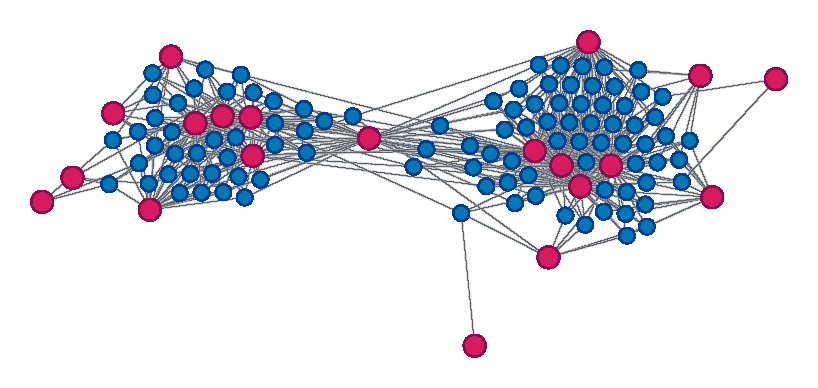
\includegraphics[width=1\linewidth,height=\textheight,keepaspectratio]{paper_files/mediabag/figures/260630-120838_A100_M5_tmax100_op1_FS_seed354_gpt_t100.pdf}

}

\caption{\label{fig-twobubbles}Snapshot of a simulation run at \(t=100\)
with agents (blue) and the statements (red) they have in memory.
Simulation with feed posting and social posting under openmindedness set
to 1 and a maximal number of 5 statements in agents' memories. (Run ID:
260630-120838\_A100\_M5\_tmax100\_op1\_FS\_seed354\_gpt\_t100)}

\end{figure}%

Figure~\ref{fig-twobubbles}, Figure~\ref{fig-libbubble}, and
Figure~\ref{fig-authbubble} show some typical outcomes we observe across
simulation runs. These figures show bipartite networks where agents
(blue) are linked to statements (red) and which are generated using a
layout computed dynamically with a version of the force-directed
algorithm \citep{FruchtermanReingold1991GraphDrawingForcedirected}. A
link means that an agent holds the statement in memory, or it integrated
this statement to its worldview. A \emph{bubble} is a group of agents
with very similar worldviews, built from a few statements that agents
outside the group rarely hold. Figure~\ref{fig-twobubbles} shows the
agent-statement network at the final step of a simulation run in which
agents could hold up to five statements in their memory and
openmindedness parameter set to 1. This result features a two-bubbles
situation where two groups of agents with different ideological leanings
(conservative/traditional vs.~liberal/progressive) emerged during the
simulation and persisted until the end of the run.

\begin{figure}[!h]

\centering{

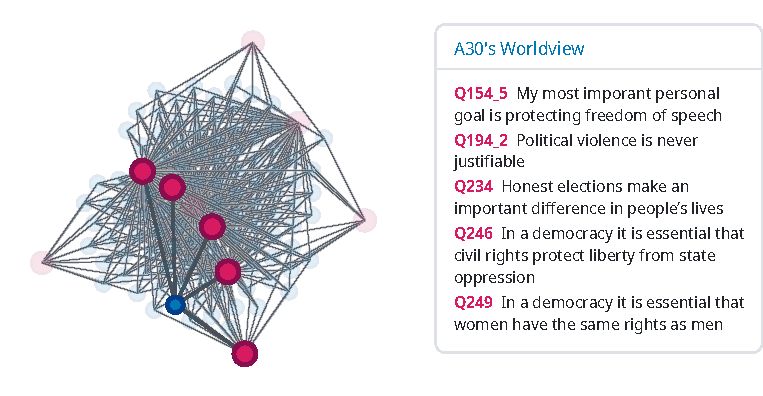
\includegraphics[width=0.7\linewidth,height=\textheight,keepaspectratio]{paper_files/mediabag/figures/260630-101930_A100_M5_tmax100_op1_FS_seed354_gpt_t100.pdf}

}

\caption{\label{fig-libbubble}Snapshot of a simulation run at \(t=100\)
analog to Figure~\ref{fig-twobubbles} using the same initial condition
but different random feed and social posting. Highlighted is the
worldview of agent 30. (Run ID:
260630-101930\_A100\_M5\_tmax100\_op1\_FS\_seed354\_gpt)}

\end{figure}%

Figure~\ref{fig-libbubble} and Figure~\ref{fig-authbubble} show a
closeup look to a specific agent's memory in two runs with identical
experimental configurations and initial conditions. An agent's worldview
trajectory may differ across such constant configuration and initial
conditions settings, because LLMs are not deterministic. Different LLM
decisions in early time steps may cause divergence between agent's
behaviors across two identical runs. Because of that, we execute three
runs with the same random seed and unique experimental configuration.
The societies in these two examples can be essentially characterized as
a consensus bubble where almost all agents are linked to a small set of
statements. While these two runs with identical parameters both ended up
in a consensus-like situation, a closeup look to a specific agent's
memory (agent 30) shows that in one of the runs this agent finished with
a freedom and equality oriented liberal worldview, while it finished
with a more security oriented conservative worldview. Snapshots of all
our simulations are available
\citep{LorenzGunes2026JanlorenzFilter_bubbles_llmLogging}.

\begin{figure}[!h]

\centering{

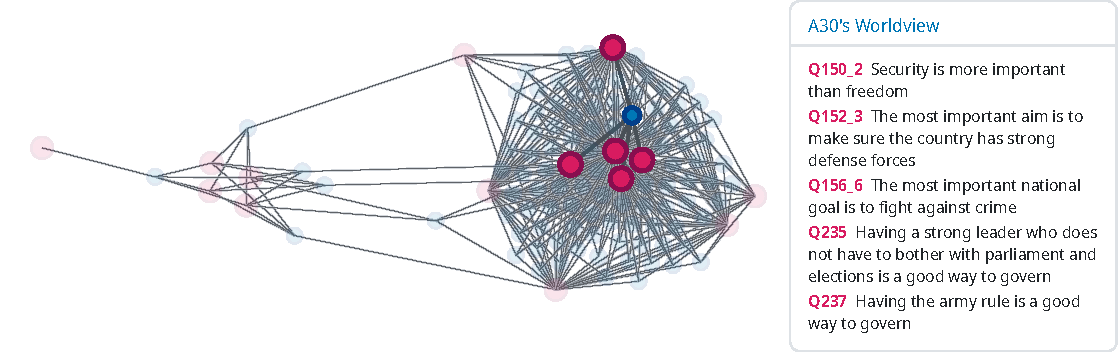
\includegraphics[width=1\linewidth,height=\textheight,keepaspectratio]{paper_files/mediabag/figures/260630-141000_A100_M5_tmax100_op1_FS_seed354_gpt_t100.pdf}

}

\caption{\label{fig-authbubble}Snapshot of a simulation run at \(t=100\)
analog to Figure~\ref{fig-twobubbles} using the same initial condition
but different random feed and social posting. Highlighted is the
worldview of agent 30. (Run ID:
260630-120838\_A100\_M5\_tmax100\_op1\_FS\_seed354\_gpt\_t100)}

\end{figure}%

To place statements on a one dimensional ideology scale, we ran a
principal component analysis (PCA) on the responses of all WVS
respondents in year 2018 (N = 33926). PCA condenses correlated answers
into a few underlying dimensions. The first principal component explains
13.5\% of the variance and is highly correlated with respondents'
left-right self-placement (r = 0.82), so we interpret it as an
ideological dimension. We asked an LLM (gpt-5.4) to classify the 100
statements into conservative and progressive categories. LLM's
classification mostly overlaps with the first principal component, and
disagreements mostly occur near zero. A comparison of PCA results and
LLM classification can be seen in Figure~\ref{fig-PCA-WVS-statements}.

\begin{figure}[!h]

\centering{

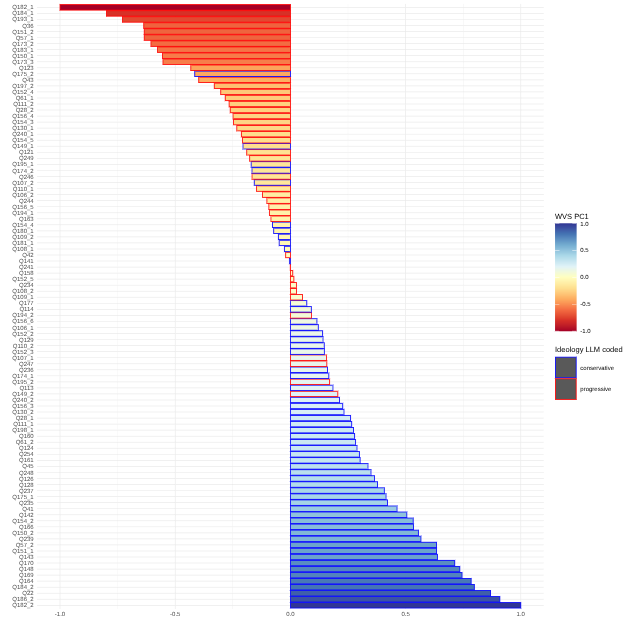
\includegraphics[width=1\linewidth,height=\textheight,keepaspectratio]{figures/fig-PCA-WVS-statements.png}

}

\caption{\label{fig-PCA-WVS-statements}1st Principal component for all
statement based on World Values Survey data.}

\end{figure}%

In Figure~\ref{fig-statement-popularity}, we show how often each
statement is part of a worldview at \emph{t=100} over all simulation
runs and parameter settings. The four most popular statements (Q246,
Q249, Q234, Q154\_5) concern civil rights, equal rights for women,
honest elections, and freedom of speech. They form the core of the
liberal bubble and lie close to the center of the first principal
component, meaning that WVS respondents across the political spectrum
tend to endorse them. Statements popular in an authoritarian bubble
reach medium popularity, while strongly conservative statements on
religion and traditional morality are rarely retained.

\begin{figure}[!h]

\centering{

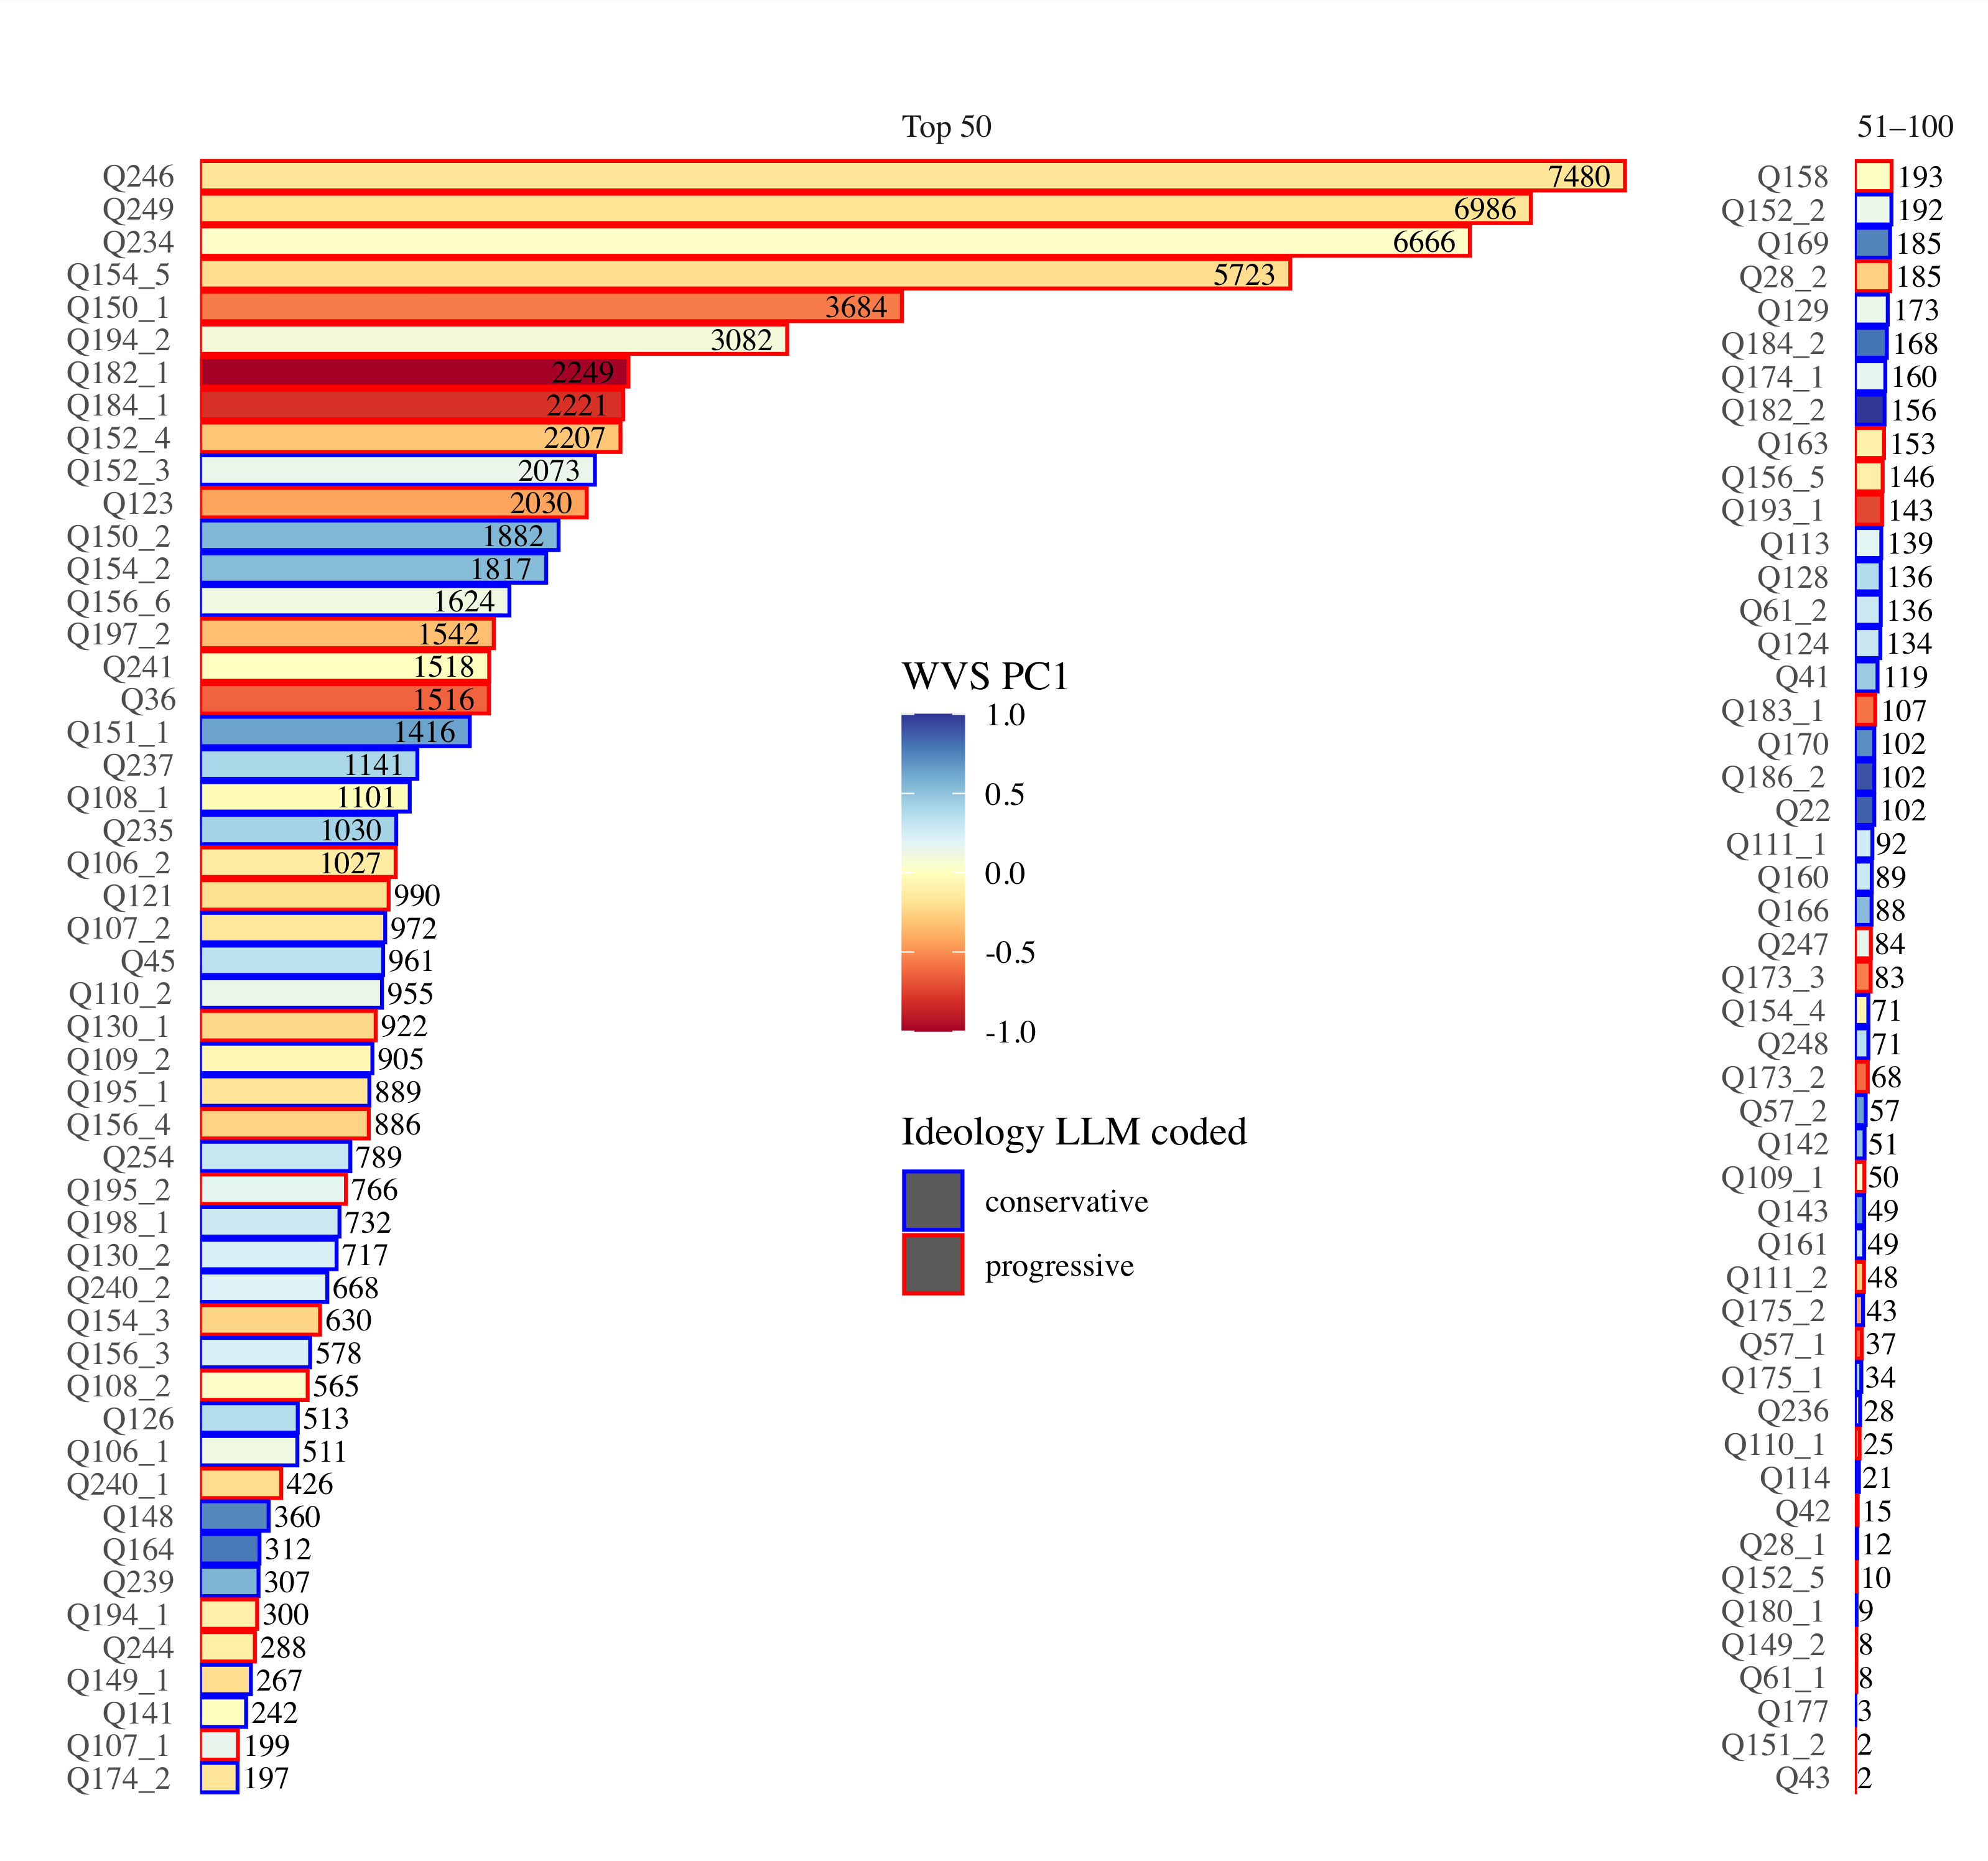
\includegraphics[width=1\linewidth,height=\textheight,keepaspectratio]{figures/fig-statement-popularity.png}

}

\caption{\label{fig-statement-popularity}Popularity of statements at
time step 100.}

\end{figure}%

Figure~\ref{fig-numstatements-per-run-plot} shows two indicators of
convergence: the number of distinct statements left at the final time
step, and the number of statements held by more than 40 agents. Social
posting clearly drives convergence, as evidenced by the drop in distinct
number of statements. With feed posting only, 47.5 statements survive on
average, compared to 24.8 with both channels and 12.6 with social
posting only. Social posting-only yields the most statements shared by
more than 40 agents, especially with memory size 10. Feed-only runs keep
a long tail of statements that vanish entirely under social posting-only
configuration.

\begin{figure}[!h]

\centering{

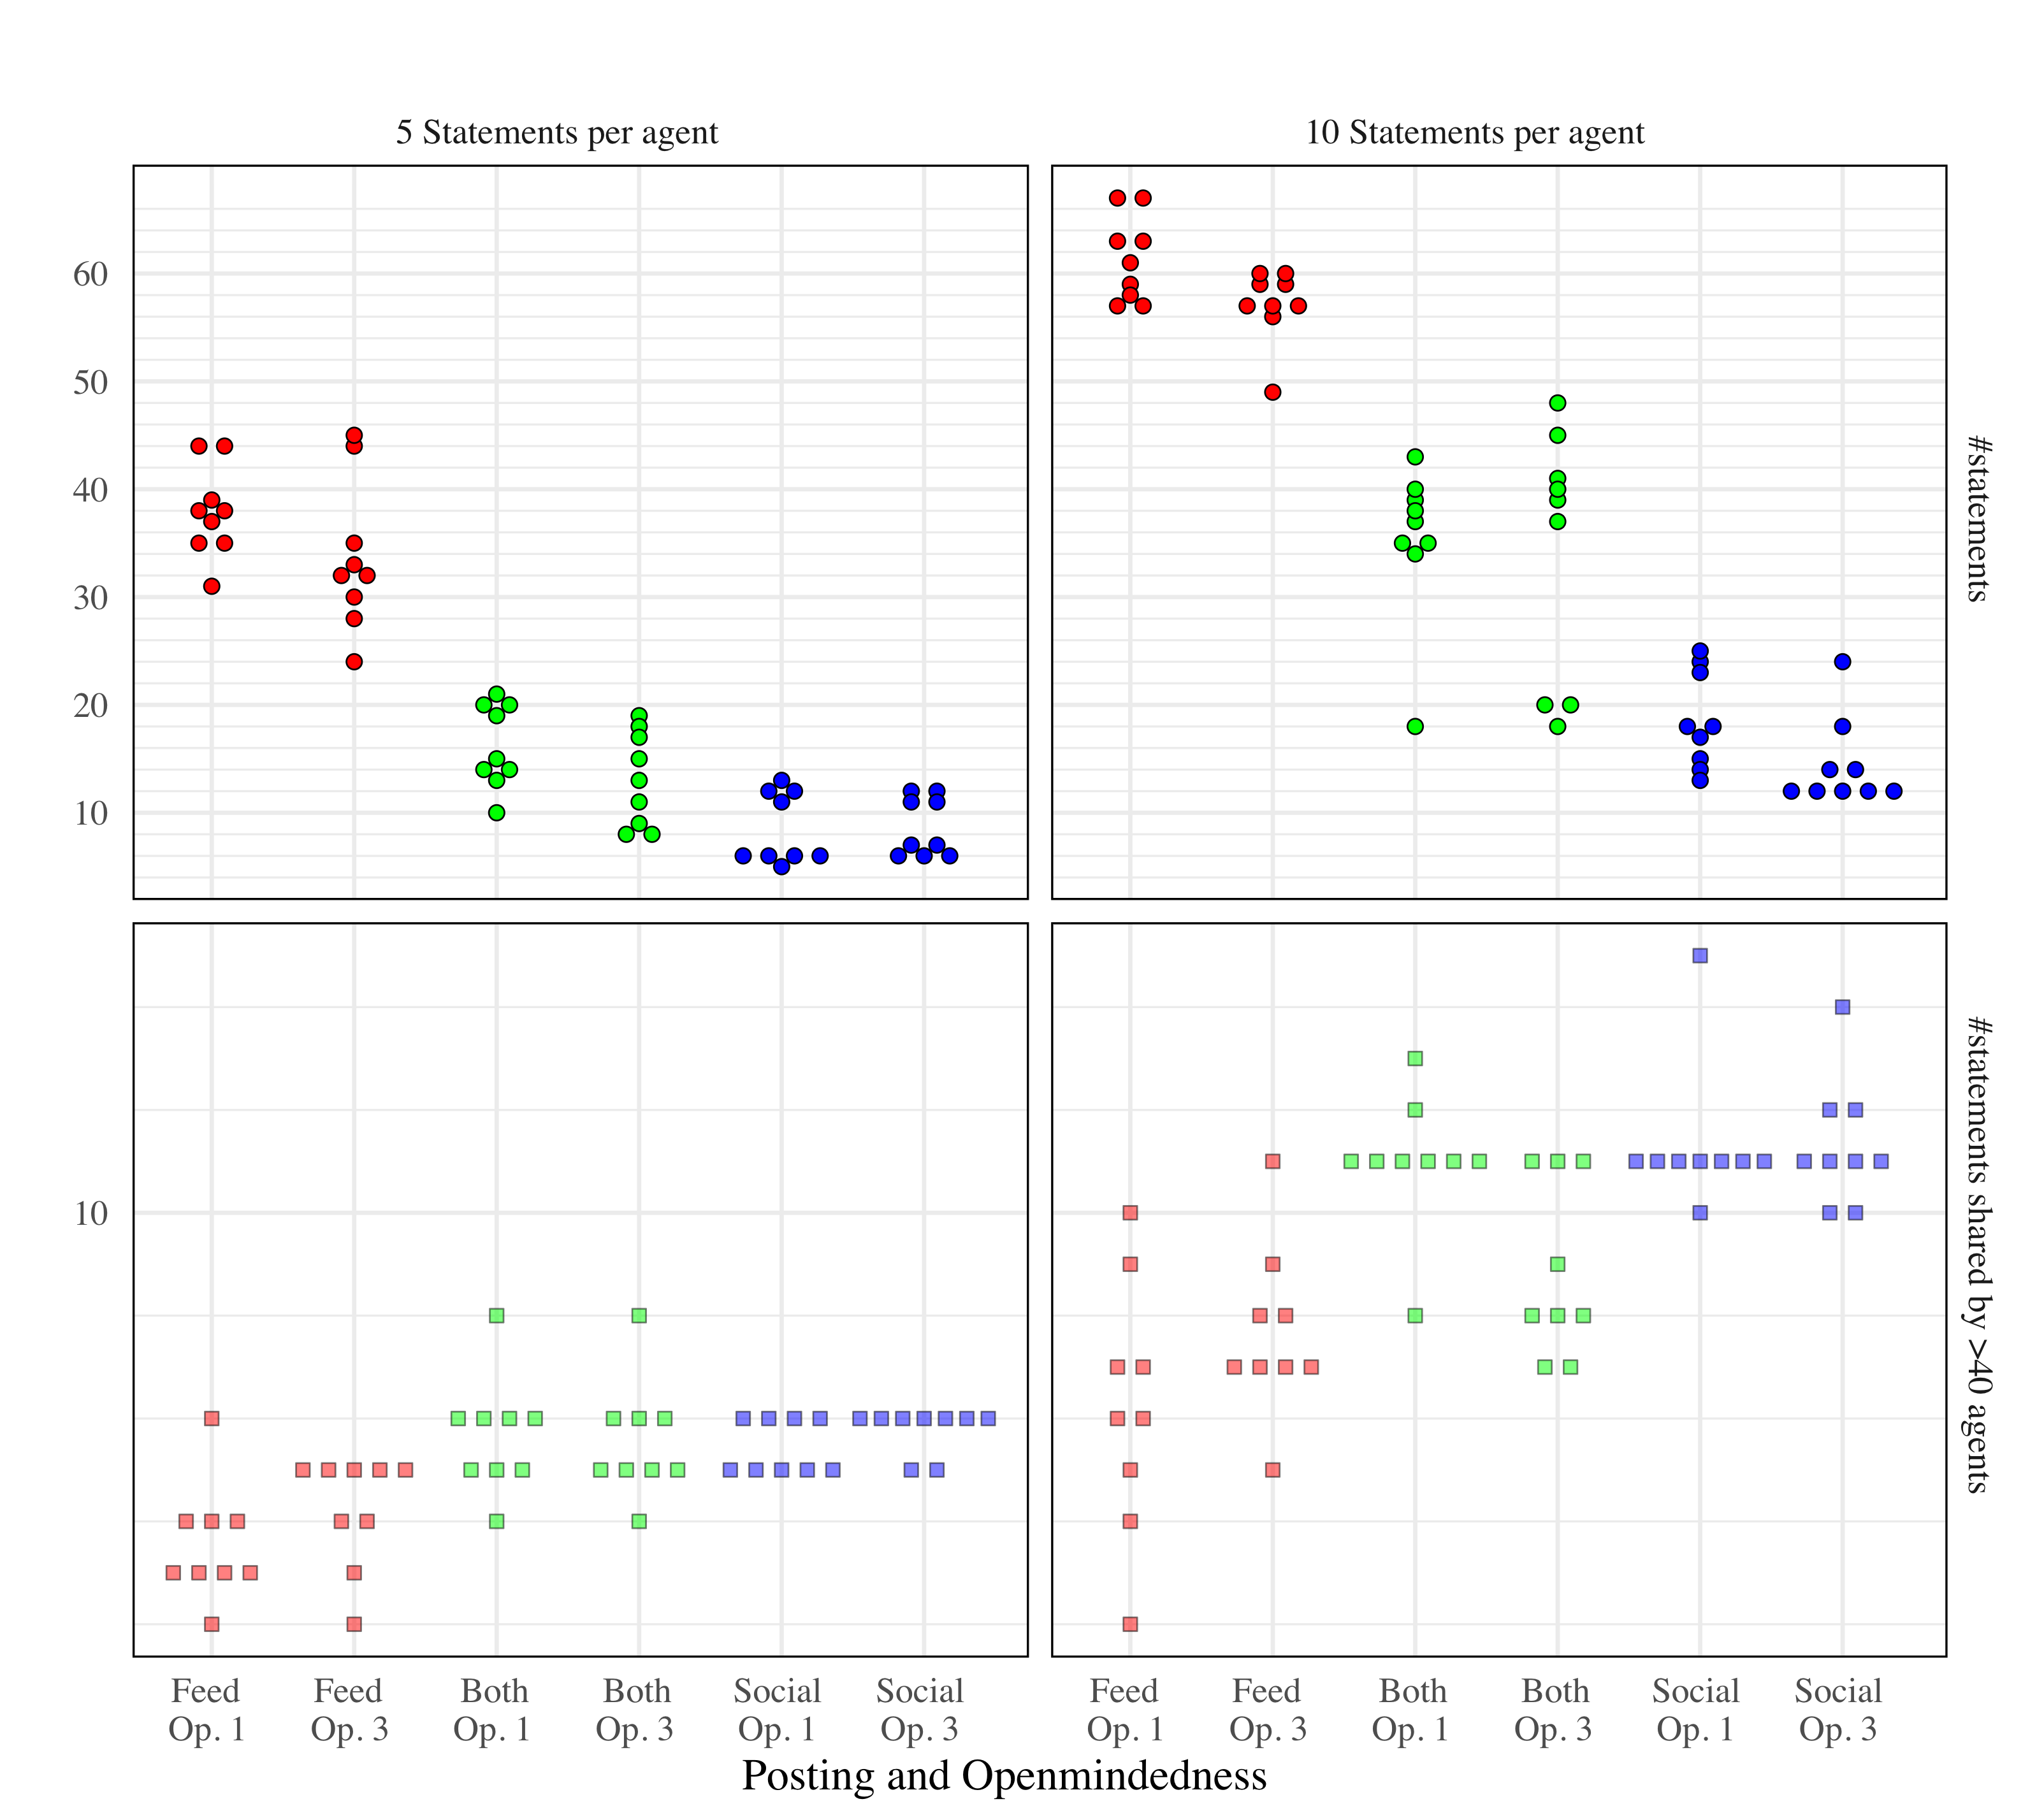
\includegraphics[width=1\linewidth,height=\textheight,keepaspectratio]{figures/fig-numstatements-per-run-plot.png}

}

\caption{\label{fig-numstatements-per-run-plot}Number of statements per
simulation run at t=100. The top row of facets shows for all runs the
total number of statements in the worldviews of all agents. The bottom
row shows for the same runs the number of very popular statements which
are shared by more than 40 agents (that means is 40\% in all runs).}

\end{figure}%

Figure~\ref{fig-wvs-sections} groups statements by the WVS questionnaire
sections of their source question and tracks each section's share of
memory slots over 100 time steps. These sections divide questions into
thematic categories, such as economic values, religious values, or
political culture and regimes, and our statements cover 12 of the 13
sections available in the WVS questionnaire. At the initialization,
statements are drawn randomly in all posting modes, so the shares of
thematic categories mirror their distribution in the statement pool.
Political culture and regimes grows from 13\% of the pool to 28\% of
memory slots at the final time step, the post-materialist values theme
from 12\% to 21\%, and political participation from 1\% to 9\%. On the
other hand, religious values category shrinks from 10\% to 1.5\%, and
some categories almost vanish.

\begin{figure}[!h]

\centering{

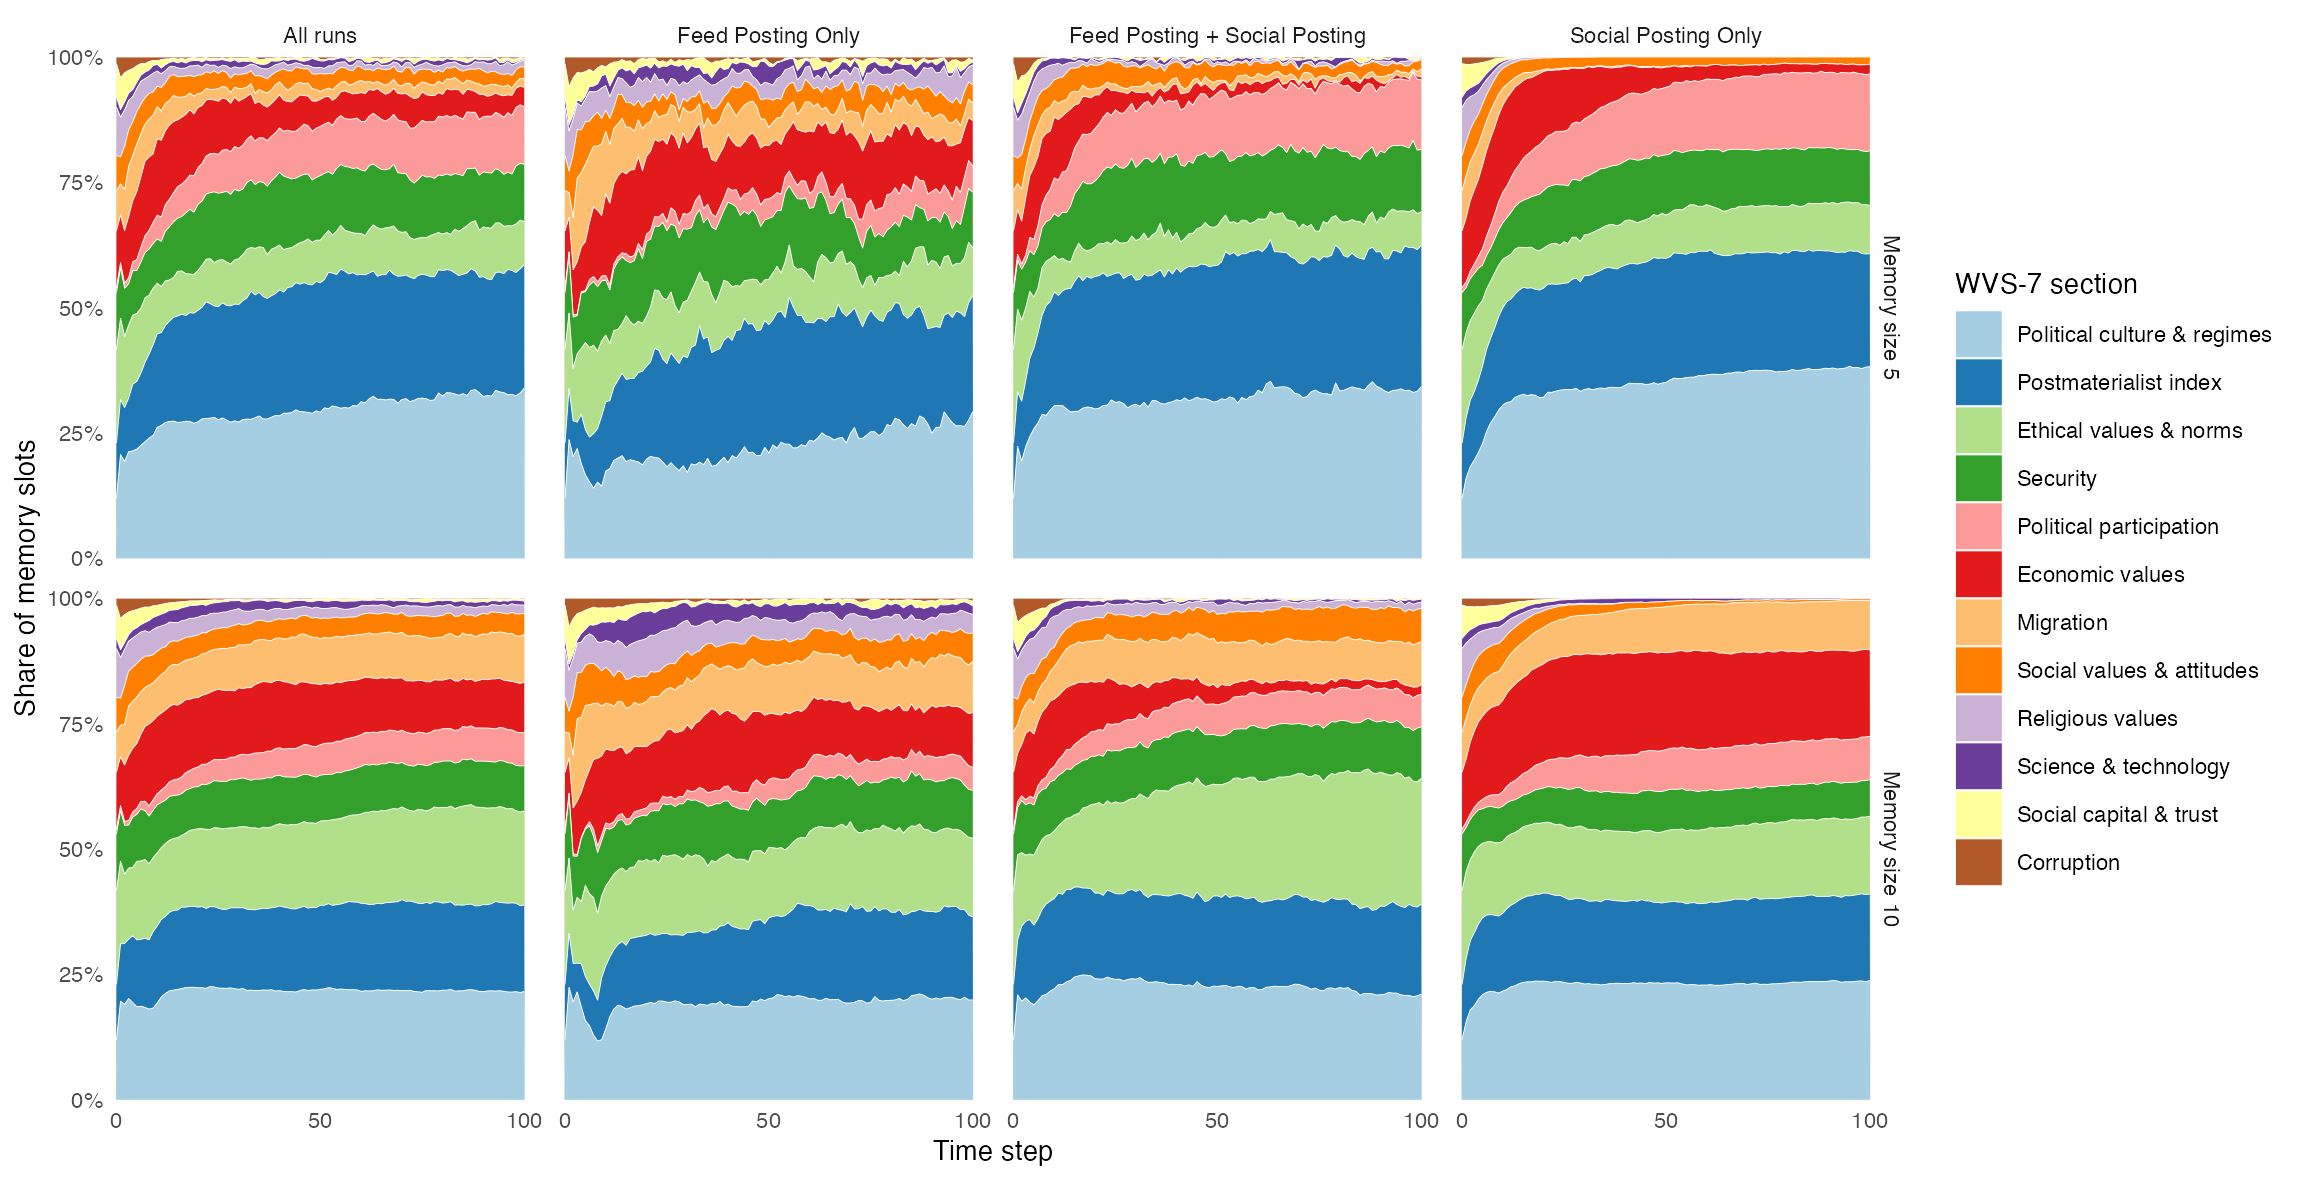
\includegraphics[width=1\linewidth,height=\textheight,keepaspectratio]{figures/fig_thematic-dist.png}

}

\caption{\label{fig-wvs-sections}Composition of agents' memories by WVS
questionnaire section over time steps, as the mean share of memory slots
across runs. Columns show all runs and the three information channel
settings. Rows show memory size 5 (top) and 10 (bottom).}

\end{figure}%

This shift hints at a thematic bias exhibited by the gpt-oss-20b model.
This bias appears even with feed-posting only, where all agents see same
statements, drawn randomly with equal probability from the statement
pool. Social posting amplifies the effect, and it is linked to the
convergence shown in Figure~\ref{fig-numstatements-per-run-plot}. As
social posting reduces the number of statements in circulation over time
steps, themes that the model rarely selects disappear first. For
example, religious values disappear in all runs with social
posting-only, while security, which has the same number of statements in
the pool, survives in two-thirds of them.

\section{Conclusion}\label{conclusion}

Our LLM-based simulations qualitatively reproduce key findings of the
original numerical model \citep{GeschkeEtAl2019TriplefilterBubbleUsing}.
We observe the emergence of worldview bubbles, which are groups of
agents sharing very similar statements that other agents rarely hold.
Social posting spurs their formation. Bubbles also appear under feed
posting alone but are less pronounced. Higher openmindedness makes a
single bubble more likely, but its effect on the number of surviving
statements is small, possibly because the model gives little weight to
our numerical operationalization of openmindedness.

The LLM version of the opinion dynamics simulation adds some features
and capabilities that numerical models lack. In the LLM version, agents
read statements in natural language and decide based on their meaning.
The LLM-based simulation shows not only whether bubbles form, but also
which worldviews they contain and which topics they cover. Linking each
statement to a survey question also allows comparing the emerging
worldviews with human attitudes. A future analysis in this direction
should clarify to what degree the emerging worldview distributions match
what we see in the in the World Values Survey, and if deviations are
caused by LLM biases or our simulation setup. Later, we plan to extend
the model to include statement generation.

\section*{Appendix}\label{appendix}
\addcontentsline{toc}{section}{Appendix}

\subsection{Prompt Example}\label{sec-prompt}

\begin{quote}
You are an individual with a worldview represented by a list of
statements. You are presented with a list of new statements coming to
your attention. Choose the single statement that best fits with your
worldview, or reject all of them if no statement fits well with your
worldview. Your list of statements is considered full when it contains
10 statements. Respond in JSON with two entries:
\texttt{selected\_statement} must be the index number of the new
statement you choose, or \texttt{None} if you do not select any
statement because they all do not fit well with your worldview.
\texttt{drop\_statement} must be the index number of the statement you
will drop from your list of worldview statements if your memory is full,
or \texttt{None} if you do not need to drop a statement. For example, if
there are three new statements shown, then the value of the
\texttt{selected\_statement} entry must be 1, 2, 3, or \texttt{None}. On
a scale from 0 to 10, where 0 means you almost never accept new
statements and 10 means you almost always accept new statements, your
openmindedness is 3.

Here are the statements you can choose from:

\begin{enumerate}
\def\labelenumi{\arabic{enumi}.}
\tightlist
\item
  ``Government should take more responsibility to ensure everyone is
  provided for''
\item
  ``Science and technology are making our lives healthier, easier, and
  more comfortable''
\item
  ``We depend too much on science and not enough on faith''
\end{enumerate}

Here is the list of your existing worldview statements:

\begin{enumerate}
\def\labelenumi{\arabic{enumi}.}
\tightlist
\item
  ``Honest elections make an important difference in people's lives''
\item
  ``Homosexuality should be treated as totally normal''
\item
  ``My most imporant personal goal is protecting freedom of speech''
\item
  ``Political violence is never justifiable''
\item
  ``The government should not monitor emails and Internet
  communication''
\item
  ``In a democracy it is essential that women have the same rights as
  men''
\item
  ``Freedom is more important than security''
\item
  ``In a democracy it is essential that civil rights protect liberty
  from state oppression''
\item
  ``Homosexual couples are as good parents as other couples.''
\item
  ``Abortion should be legal''
\end{enumerate}
\end{quote}

This particular prompt resulted in the outcome:

Agent selected: ``Science and technology are making our lives healthier,
easier, and more comfortable''

Agent dropped: ``The government should not monitor emails and Internet
communication''

\subsection{Statement Pool}\label{statement-pool}

\begingroup
\setlength\LTleft{0\linewidth}
\setlength\LTright{0\linewidth}\fontsize{12.0pt}{14.0pt}\selectfont

\begin{longtable}{@{\extracolsep{\fill}}l>{\raggedright\arraybackslash}p{\dimexpr 0.70\linewidth -2\tabcolsep-1.5\arrayrulewidth}l}

\caption{\label{tbl-statements}The hundred statements used as statement
pools. \emph{id} refers to the question code in the World Values Survey
questionaire. The numeric suffix of \emph{id} labels different
statements derived from the same question.}

\tabularnewline

\toprule
id & statement & worldview \\ 
\midrule\addlinespace[2.5pt]
Q22 & I would not like to have homosexuals as neighbors. & conservative \\ 
Q28\_1 & When a mother works for pay, children suffer. & conservative \\ 
Q28\_2 & When a mother works for pay, children benefit. & progressive \\ 
Q36 & Homosexual couples are as good parents as other couples. & progressive \\ 
Q41 & Work should always come first, even if it means less spare time. & conservative \\ 
Q42 & Our society must be radically changed by revolutionary action. & progressive \\ 
Q43 & Less importance placed on work in the future would be a good thing & progressive \\ 
Q45 & Greater respect for authority in the future would be a good thing & conservative \\ 
Q57\_1 & Most people can be trusted & progressive \\ 
Q57\_2 & I am very careful in putting trust in other people. & conservative \\ 
Q61\_1 & I trust people I meet for the first time & progressive \\ 
Q61\_2 & I do not trust people I meet for the first time & conservative \\ 
Q106\_1 & Larger income differences should be accepted to reward individual effort & conservative \\ 
Q106\_2 & Incomes should be more equal & progressive \\ 
Q107\_1 & Government ownership of business should be increased & progressive \\ 
Q107\_2 & Private ownership of business should be increased & conservative \\ 
Q108\_1 & People should take more responsibility to provide for themselves & conservative \\ 
Q108\_2 & Government should take more responsibility to ensure everyone is provided for & progressive \\ 
Q109\_1 & Competition is harmful & progressive \\ 
Q109\_2 & Competition is good & conservative \\ 
Q110\_1 & Success in life depends more on luck and connections than hard work & progressive \\ 
Q110\_2 & Hard work brings a better life & conservative \\ 
Q111\_1 & Economic growth should be prioritized even if it harms the environment & conservative \\ 
Q111\_2 & Environmental protection should be prioritized even if it harms economic growth & progressive \\ 
Q113 & Most state authorities are involved in corruption & progressive \\ 
Q114 & Most or all business executives are involved in corruption & progressive \\ 
Q121 & Immigrants have a positive impact on the development of the country & progressive \\ 
Q123 & Immigrants strengthen cultural diversity & progressive \\ 
Q124 & Immigrants increase the crime rate & conservative \\ 
Q126 & Immigrants increase the risks of terrorism & conservative \\ 
Q128 & Immigrants increase unemployment & conservative \\ 
Q129 & Immigrants lead to social conflict & conservative \\ 
Q130\_1 & The government should let anyone from other countries come here who wants to work & progressive \\ 
Q130\_2 & The government should prohibit people from other countries coming here & conservative \\ 
Q141 & I carry a knife, gun, or weapon for protection & conservative \\ 
Q142 & I am worried about losing or not finding a job & progressive \\ 
Q143 & I am worried about not giving my children a good education & progressive \\ 
Q148 & I am very worried about a civil war & progressive \\ 
Q149\_1 & Freedom is more important than equality & conservative \\ 
Q149\_2 & Equality is more important than freedom & progressive \\ 
Q150\_1 & Freedom is more important than security & progressive \\ 
Q150\_2 & Security is more important than freedom & conservative \\ 
Q151\_1 & I would be willing to fight for my country & conservative \\ 
Q151\_2 & I am not willing to fight for my country & progressive \\ 
Q152\_2 & The most important aim for the country is high economic growth & conservative \\ 
Q152\_3 & The most important aim is to make sure the country has strong defense forces & conservative \\ 
Q152\_4 & The most important aim for the country is that people have more say about how things are\newline done at their jobs and in their communities & progressive \\ 
Q152\_5 & The most important aim for the country is to make cities and countryside more beautiful & progressive \\ 
Q154\_2 & My most imporant personal goal is to maintain order in the country & conservative \\ 
Q154\_3 & My most imporant personal goal is to have more say in important government decisions & progressive \\ 
Q154\_4 & My most imporant personal goal is fighting rising prices & conservative \\ 
Q154\_5 & My most imporant personal goal is protecting freedom of speech & progressive \\ 
Q156\_3 & The most important national goal is a stable economy & conservative \\ 
Q156\_4 & The most important national goal a more humane society & progressive \\ 
Q156\_5 & The most important national goal is that ideas count more than money & progressive \\ 
Q156\_6 & The most important national goal is to fight against crime & conservative \\ 
Q158 & Science and technology are making our lives healthier, easier, and more comfortable & conservative \\ 
Q160 & We depend too much on science and not enough on faith & conservative \\ 
Q161 & One of the bad effects of science is that it breaks down people’s ideas of right and wrong & conservative \\ 
Q163 & The world is better off because of science and technology & progressive \\ 
Q164 & God is very important in my life & conservative \\ 
Q166 & I believe in life after death & conservative \\ 
Q169 & Whenever science and religion are in conflict, religion is right & conservative \\ 
Q170 & The only acceptable religion is my religion & conservative \\ 
Q173\_2 & I consider myself an atheist & progressive \\ 
Q173\_3 & I consider myself not religious & progressive \\ 
Q174\_1 & The meaning of religion is to follow norms and ceremonies & conservative \\ 
Q174\_2 & The meaning of religion is to do good to other people & progressive \\ 
Q175\_1 & The meaning of religion is to make sense of life after death & conservative \\ 
Q175\_2 & The meaning of religion is to make sense of life in this world & progressive \\ 
Q177 & Claiming government benefits to which you are not entitled is justifiable & progressive \\ 
Q180\_1 & Cheating on taxes if you have a chance is justifiable & progressive \\ 
Q181\_1 & Accepting a bribe in the course of duties is justifiable & progressive \\ 
Q182\_1 & Homosexuality should be treated as totally normal & progressive \\ 
Q182\_2 & Homosexuality is never justifiable & conservative \\ 
Q183\_1 & Prostitution should be legal & progressive \\ 
Q184\_1 & Abortion should be legal & progressive \\ 
Q184\_2 & Abortion is never justifiable & conservative \\ 
Q186\_2 & Sex before marriage is never justifiable & conservative \\ 
Q193\_1 & Having casual sex is OK & progressive \\ 
Q194\_1 & Political violence can be justifiable & progressive \\ 
Q194\_2 & Political violence is never justifiable & conservative \\ 
Q195\_1 & Death penalty is justifiable & conservative \\ 
Q195\_2 & Death penalty is never justifiable & progressive \\ 
Q198\_1 & The government should have the right to collect information about citizens without their knowledge & conservative \\ 
Q197\_2 & The government should not monitor emails and Internet communication & progressive \\ 
Q234 & Honest elections make an important difference in people’s lives & progressive \\ 
Q235 & Having a strong leader who does not have to bother with parliament and elections is a good way to govern & conservative \\ 
Q236 & Having experts make decisions instead of government is a good way to govern & conservative \\ 
Q237 & Having the army rule is a good way to govern & conservative \\ 
Q239 & Having a system governed by religious law without parties or elections is a good way to govern & conservative \\ 
Q240\_1 & I place myself on the left side of the political scale & progressive \\ 
Q240\_2 & I place myself on the right side of political scale & conservative \\ 
Q241 & In a democracy it is essential that governments tax the rich and subsidize the poor & progressive \\ 
Q244 & In a democracy it is essential that people receive state aid for unemployment & progressive \\ 
Q246 & In a democracy it is essential that civil rights protect liberty from state oppression & progressive \\ 
Q247 & In a democracy it is essential to make people’s incomes equal & progressive \\ 
Q248 & In a democracy it is essential that people obey their rulers & conservative \\ 
Q249 & In a democracy it is essential that women have the same rights as men & progressive \\ 
Q254 & I am proud of my nation & conservative \\ 
\bottomrule

\end{longtable}

\endgroup

\section*{Acknowledgements}\label{acknowledgements}
\addcontentsline{toc}{section}{Acknowledgements}

We acknowledge the support of the European City Squared project, funded
by the European Union's Horizon Europe research and innovation programme
under grant agreement DOI:
\href{https://doi.org/10.3030/101178170}{10.3030/101178170}. We thank
our colleagues in the project for their valuable feedback and
discussions on this work.

We thank Alua Aldaniyaz and Asmae Nakib for their data analysis of World
Value Survey. Their work also built the basis of the selection of
statements from the World Value Survey questionnaire for our model. We
thank Betül Yurtman for her work on assessing the empirical plausibility
of emerging worldviews in the LLM-based agent-based model. We thank
Tiancheng Hu for advise on designing LLM based workflows for simulating
human behavior.

\bibliographystyle{elsarticle-num-names}
\bibliography{../ABM-LLM.bib}

\end{document}
